\documentclass{article}

\usepackage{graphicx}
\usepackage{amsmath}
\usepackage{cancel}
\usepackage{polynom}
\usepackage{float}

\oddsidemargin 0in
\topmargin -0.5in
\textwidth 6.5in

\title{Math 115 Syllabus}
\date{September 21, 2010}
\author{Ed Tellman}

\begin{document}

\maketitle

\section{Introduction}
This course will cover {\em Precalculus}, by Faires and DeFranza.  It bridges the gap between algebra and calculus and
prepares you to take the Math-263 calculus sequence offered by Ohio University.

\section{Homework and Exams}
You should expect to spend a few hours each week doing homework.  You are welcome to work together on homework.
If you are having difficulty with a problem feel free to consult with another student.

Math is like learning piano, basketball, or bicycle mechanics.  Watching someone else do it or reading about it in a
book is helpful.  But you can't actually learn how to do it yourself unless you've practiced on your own.

% We won't spend any time doing homework in class.  But we will discuss some of the homework problems from the
% previous week, and answer any questions which came up.

Each chapter will be followed by an in-class examination to make sure that everyone is keeping up.

\section{Text Book}
The current edition of the text book is the fourth edition.  However, this edition costs about \$150 while older
editions, which seem to be very similar, are available used for about \$2.  So given our limited budget, we're using
the older editions.

We are ordering one copy of the current edition.  I'll make sure we cover everything it includes and use some problems
from it for homework.

\section{Calculators}
There are some problems in the text which require the use of a graphing calculator.  These aren't required for the
course and the final.  But it would be nice to be able to do some of them, so we're trying to arrange to buy some 
graphing calculators.

\section{Attendance}
I'll try to make the classes interesting and useful, so that that attending class helps you to understand the
material and do the homework.

I think the prison and UBB frown upon students who sign up for class but don't attend regularly.  If you find you are
unable to attend, let me know know and the TA and I will help you catch up on whatever you missed.

\section{Course Credit}
Anyone who is doing OK in the course and is interested in getting credit can take the Ohio University exam.
Unlike how we handled things in Math 113, we'll take care of the paper work well before the end of the course so you won't
have to wait months to take the test.

\section{Course Overview}

% Here's what we will cover in this course.  Don't worry if some of the terms are unfamiliar or the equations look
% complicated.  Mathematicians like to use imposing terms for simple concepts, as it helps their job security.  

You will probably already be somewhat familiar with some of the topics.  But this course will cover things in more
depth, so you still shouldn't be too bored, even if you've seen some of the topics before.

The first chapter provides an introduction to functions.  It defines functions and describes some common ways in which
they are combined.  After the first chapter, each chapter focuses on a different category of function.  For each type of
function, we discuss what its graph looks like, how to work with equations containing it, etc.  So each chapter is fairly
similar, aside from the specific type of function covered.

\subsection{Chapter One--Functions}
The first chapter introduces functions and ways in which they can be combined.  

\subsection{Chapter Two--Algebraic Functions}

This chapter covers functions which are formed out of $+$, $-$, $\cdot$, $\div$, and $\sqrt{\hspace{0.1cm}}$.  

Examples of algebraic functions are: $f(x) = 2x + 3$, $f(x) = (x-2)^2$, and $f(x) = \sqrt{x - 4}$

% For example:
% \begin{itemize}
%   \item $f(x) = \dfrac{1}{2} x + 2$
%   \item $f(x) = -(x-2)^2 + 4$
%   \item $f(x) = -(x+4)^3$
% \end{itemize}

\begin{figure}[H]
  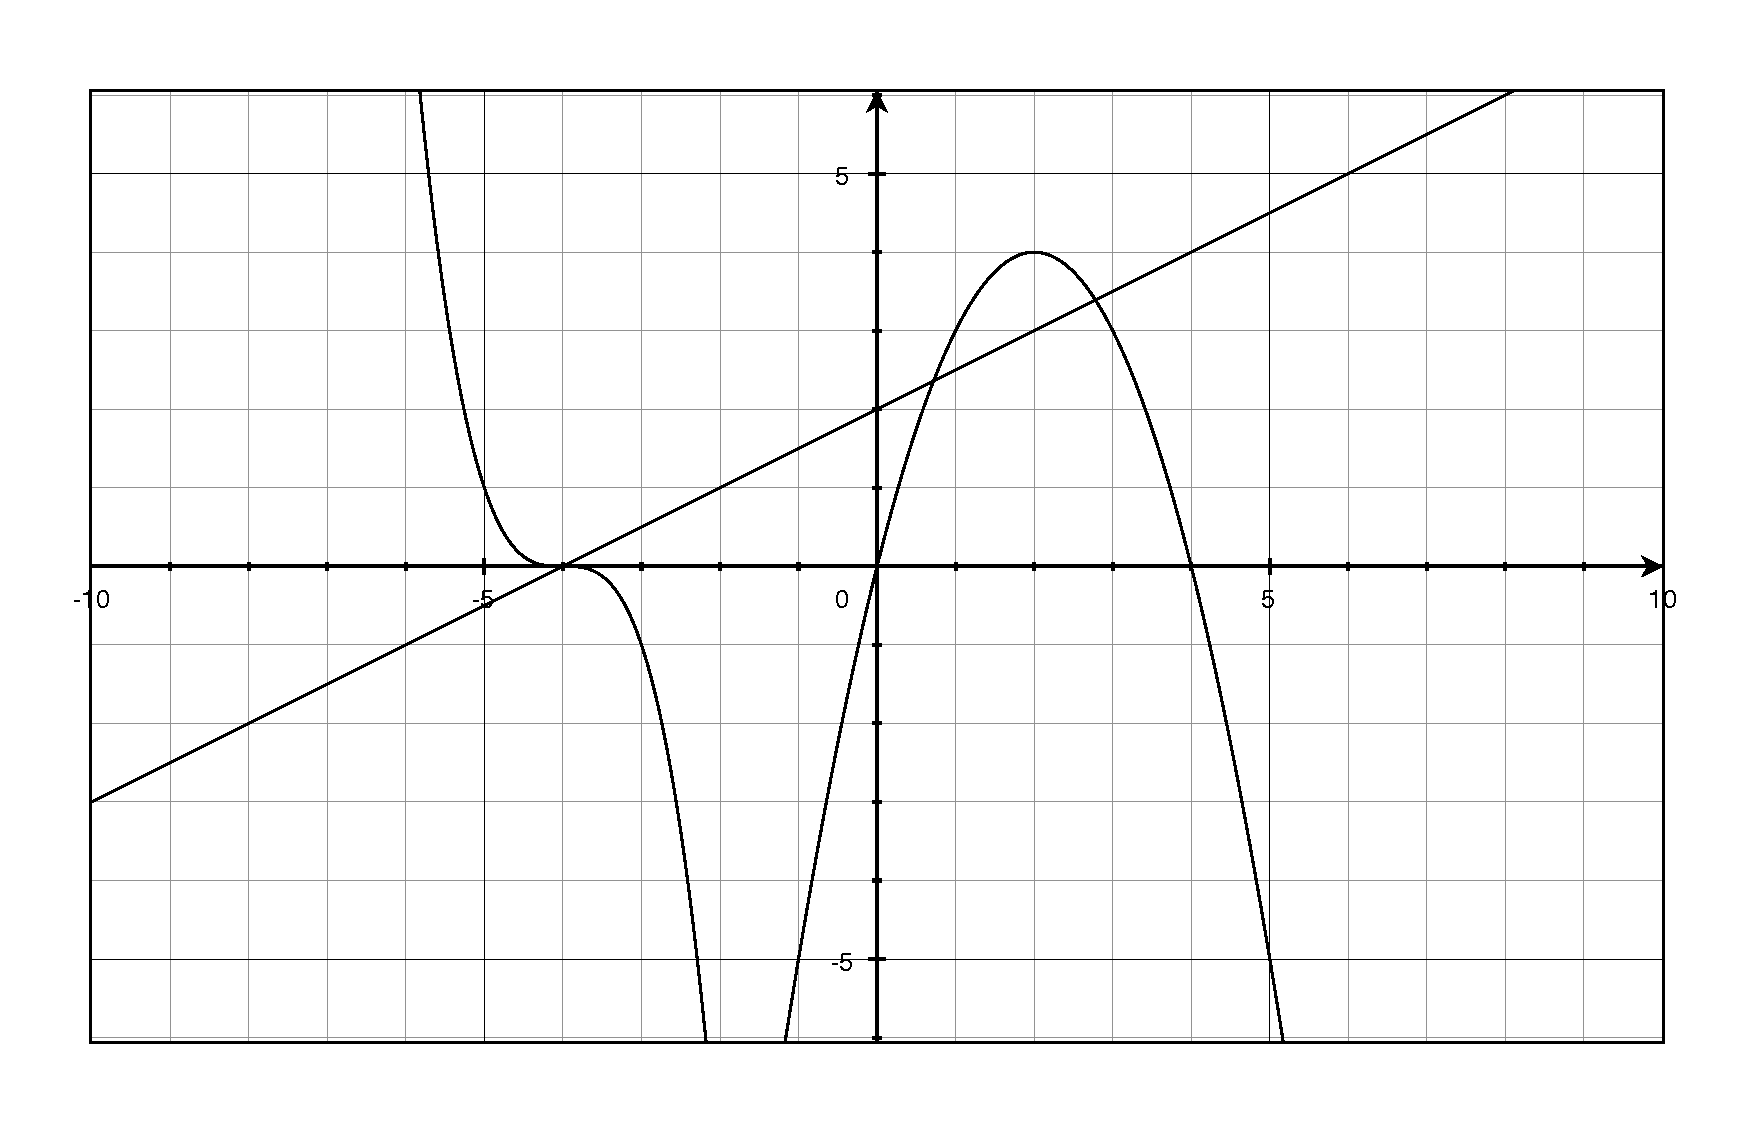
\includegraphics[width=12cm,height=7cm]{algebraic}
\end{figure}

\pagebreak

\subsection{Chapter Three--Trigonometric Functions}

This chapter covers the trigonometric functions: $sin$, $cos$, $tan$, etc.

\begin{figure}[H]
  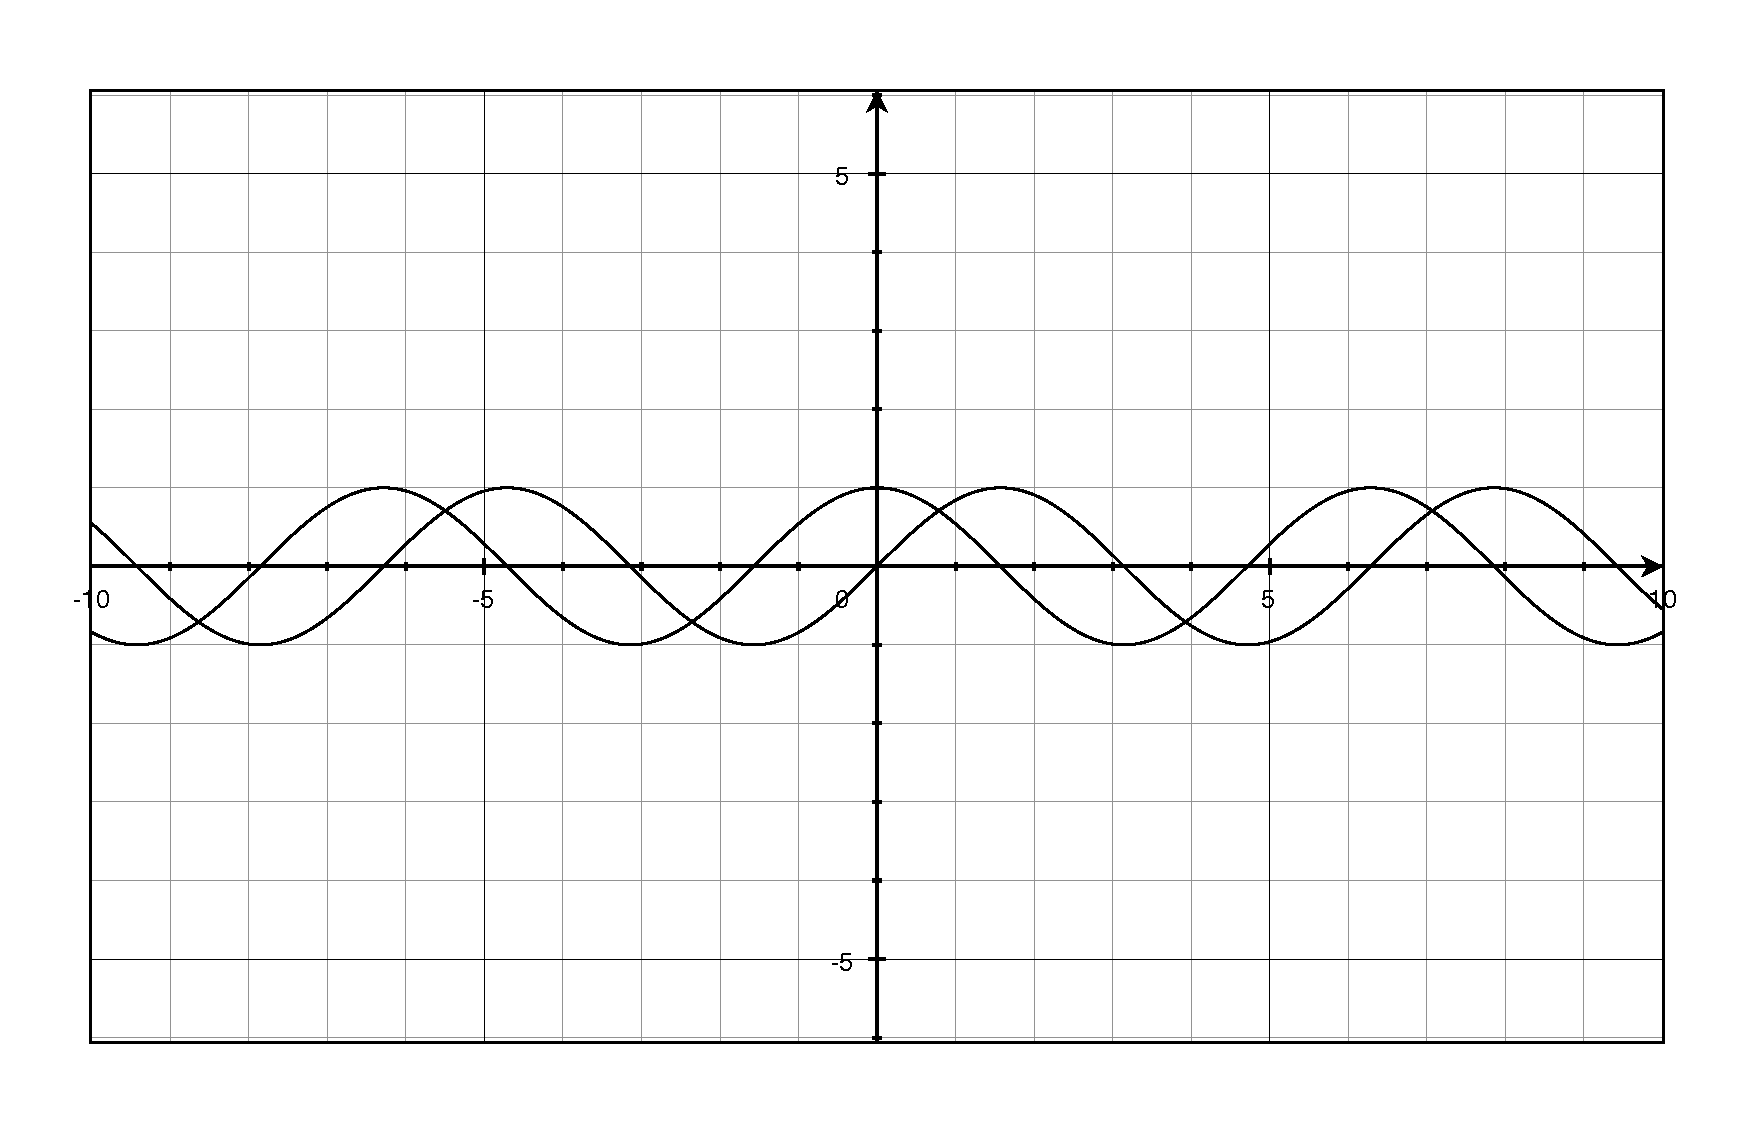
\includegraphics[width=12cm,height=7cm]{trig}
\end{figure}


\subsection{Chapter Four--Exponential and Logarithm Functions}
This chapter is covers the exponential and logarithm functions.  For example:
\begin{itemize}
  \item $f(x) = e^x$
  \item $f(x) = \ln(x)$
\end{itemize}

\begin{figure}[H]
  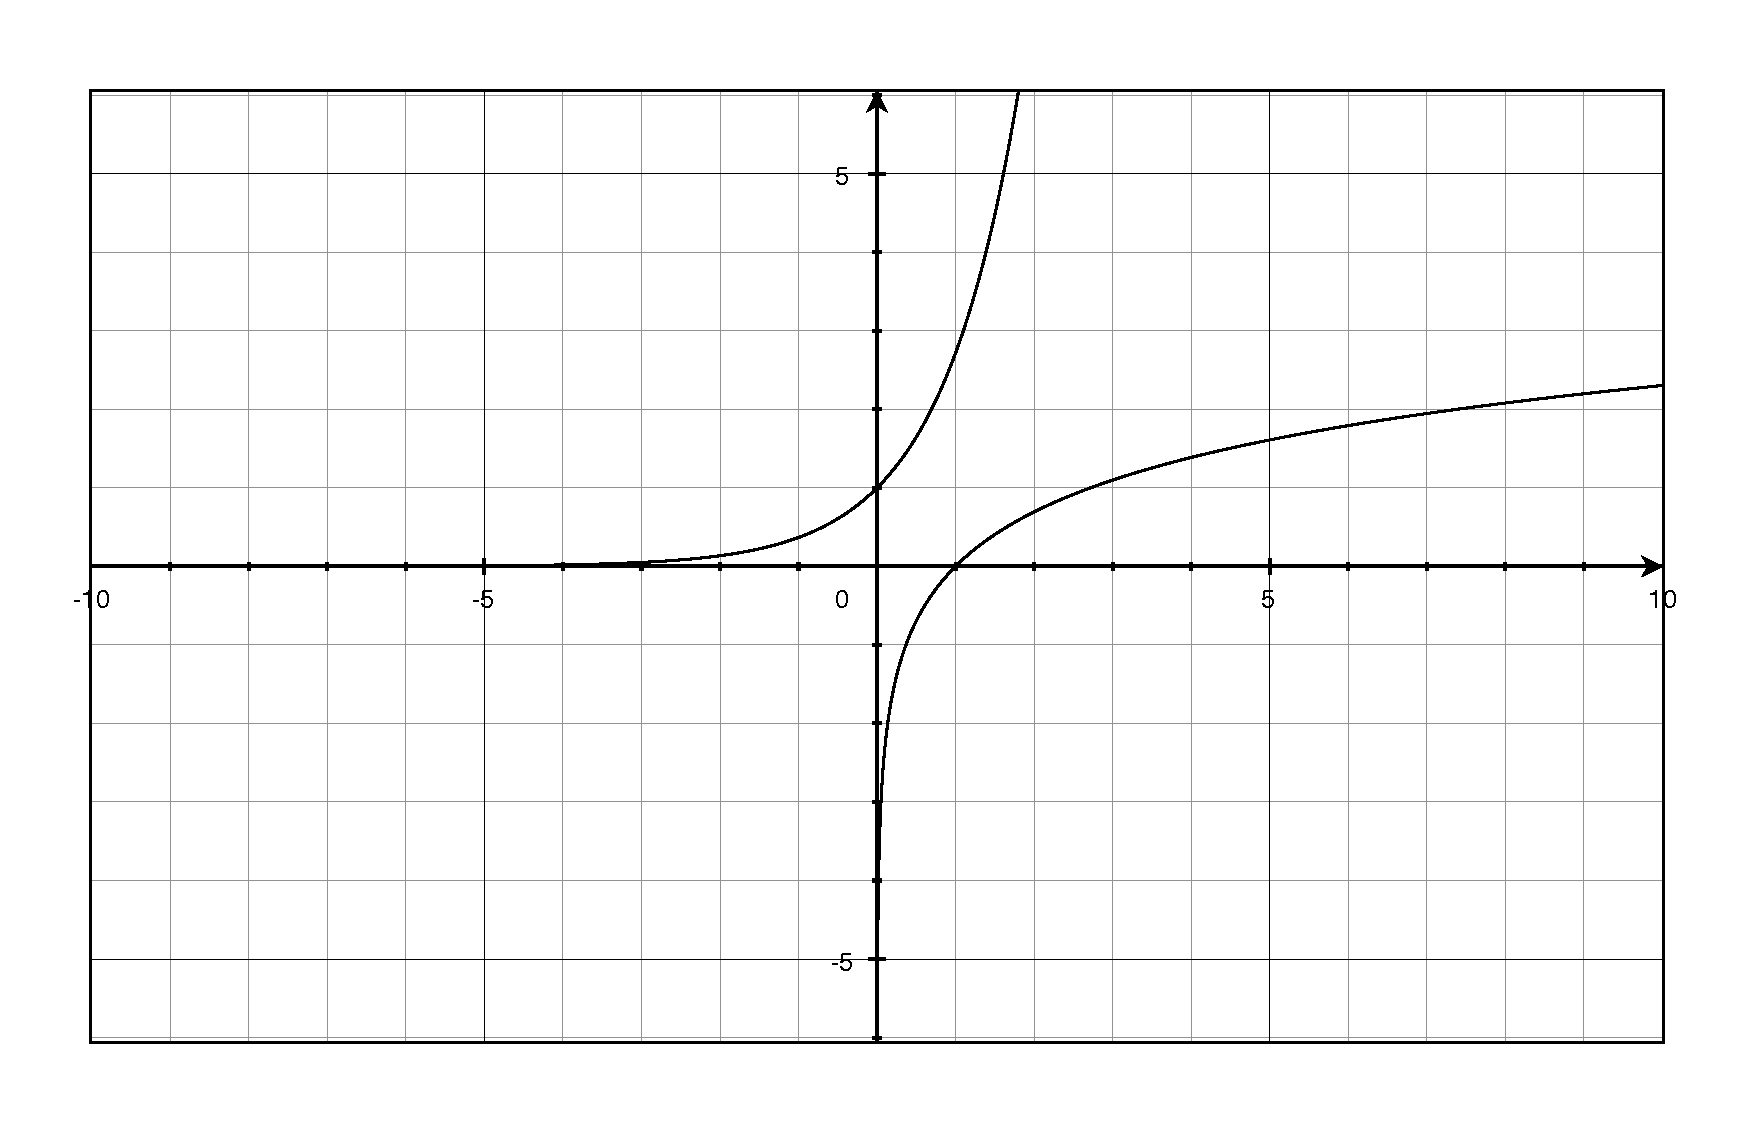
\includegraphics[width=12cm,height=7cm]{exponential}
\end{figure}

\subsection{Chapter Five--Conic Sections, Polar Coordinates, and Parametric Equations}
This chapter covers the graphs of equations for curves which occur when you cut a slice out of a cone.  This includes:
\begin{itemize}
  \item parabola: $y = x^2$
  \item ellipse: $\dfrac{x^2}{9} + \dfrac{y^2}{16} = 1$
  \item hyperbola: $\dfrac{x^2}{25} - \dfrac{y^2}{16} = 12$
\end{itemize}

\begin{figure}[H]
  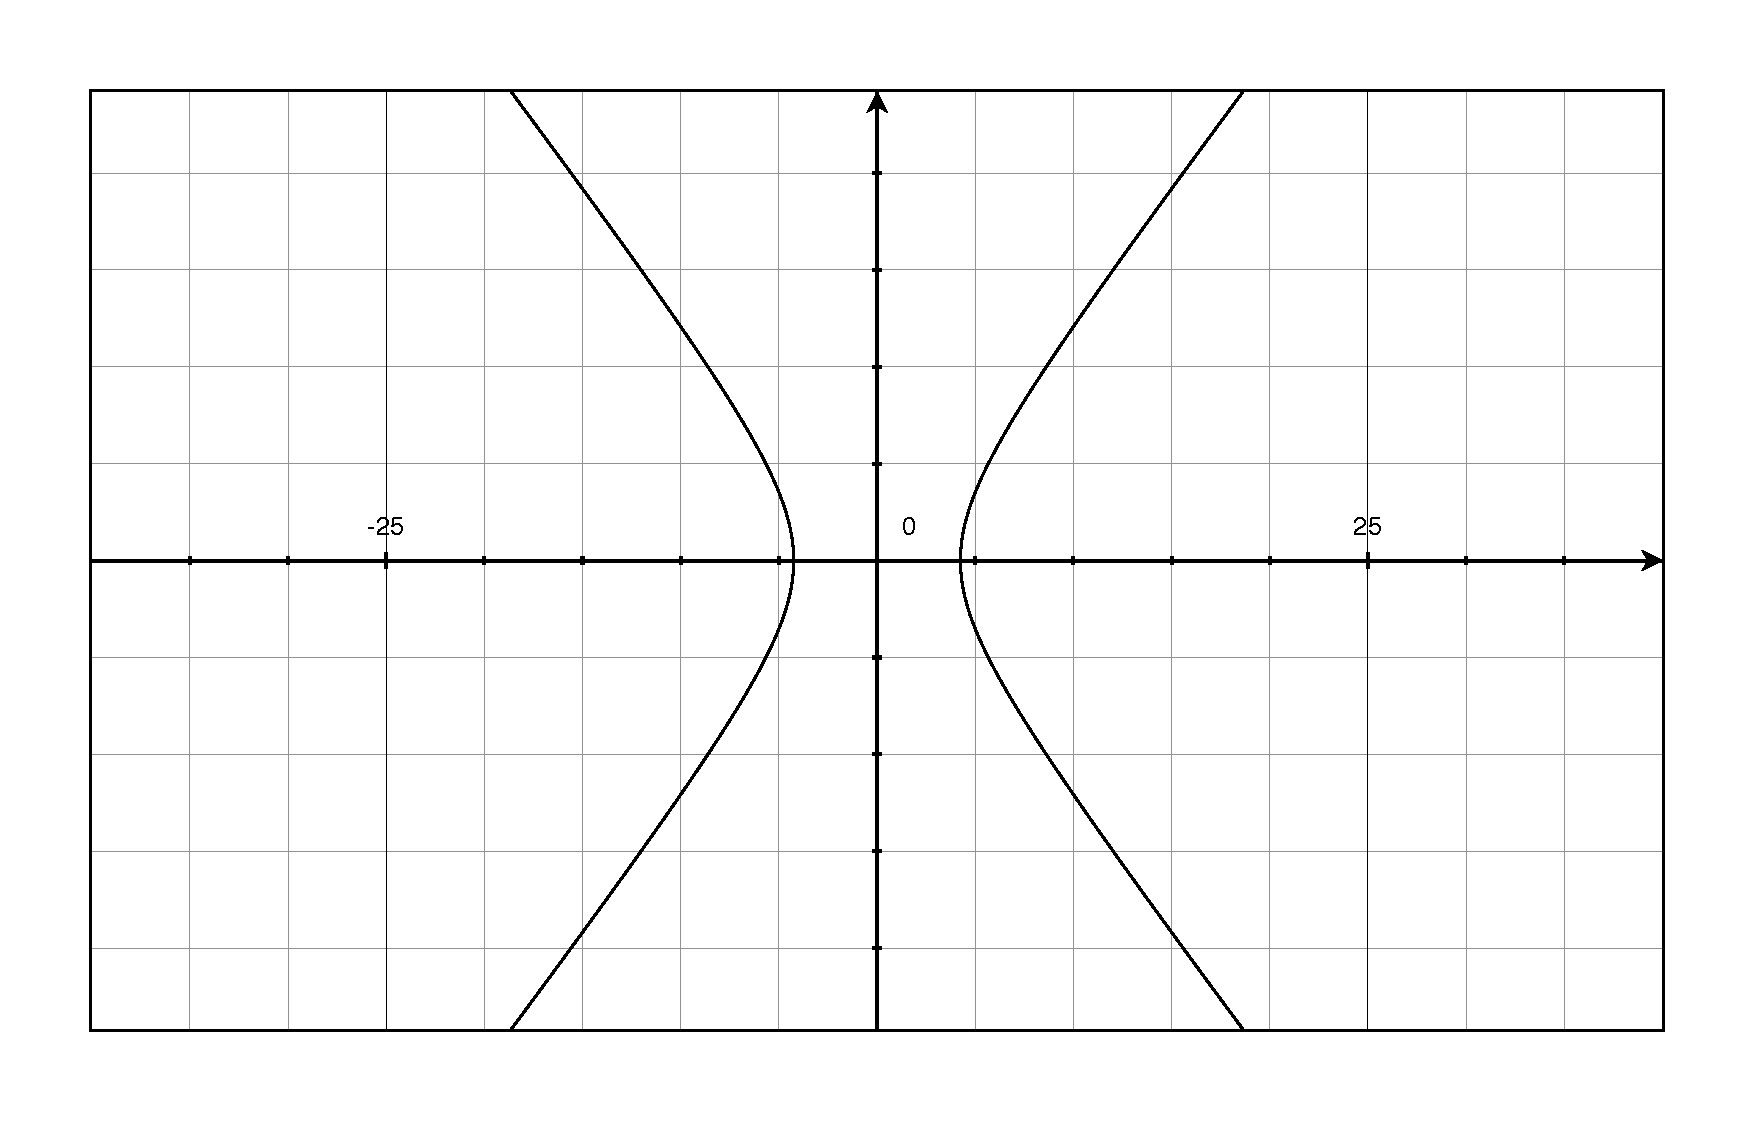
\includegraphics[width=12cm,height=7cm]{conic}
\end{figure}

\end{document}

